% Options for packages loaded elsewhere
\PassOptionsToPackage{unicode}{hyperref}
\PassOptionsToPackage{hyphens}{url}
%
\documentclass[
  17pt,
  letterpaper,
  ignorenonframetext,
  aspectratio=169,
  handout]{beamer}
\usepackage{pgfpages}
\setbeamertemplate{caption}[numbered]
\setbeamertemplate{caption label separator}{: }
\setbeamercolor{caption name}{fg=normal text.fg}
\beamertemplatenavigationsymbolsempty
% Prevent slide breaks in the middle of a paragraph
\widowpenalties 1 10000
\raggedbottom
\setbeamertemplate{part page}{
  \centering
  \begin{beamercolorbox}[sep=16pt,center]{part title}
    \usebeamerfont{part title}\insertpart\par
  \end{beamercolorbox}
}
\setbeamertemplate{section page}{
  \centering
  \begin{beamercolorbox}[sep=12pt,center]{part title}
    \usebeamerfont{section title}\insertsection\par
  \end{beamercolorbox}
}
\setbeamertemplate{subsection page}{
  \centering
  \begin{beamercolorbox}[sep=8pt,center]{part title}
    \usebeamerfont{subsection title}\insertsubsection\par
  \end{beamercolorbox}
}
\AtBeginPart{
  \frame{\partpage}
}
\AtBeginSection{
  \ifbibliography
  \else
    \frame{\sectionpage}
  \fi
}
\AtBeginSubsection{
  \frame{\subsectionpage}
}

\usepackage{amsmath,amssymb}
\usepackage{lmodern}
\usepackage{iftex}
\ifPDFTeX
  \usepackage[T1]{fontenc}
  \usepackage[utf8]{inputenc}
  \usepackage{textcomp} % provide euro and other symbols
\else % if luatex or xetex
  \usepackage{unicode-math}
  \defaultfontfeatures{Scale=MatchLowercase}
  \defaultfontfeatures[\rmfamily]{Ligatures=TeX,Scale=1}
  \setmainfont[BoldFont = SF Pro Text Semibold, Scale =
MatchLowercase]{SF Pro Text Light}
\fi
\usecolortheme{wolverine}
\usefonttheme{serif} % use mainfont rather than sansfont for slide text
\useinnertheme{default}
\useoutertheme{miniframes}
% Use upquote if available, for straight quotes in verbatim environments
\IfFileExists{upquote.sty}{\usepackage{upquote}}{}
\IfFileExists{microtype.sty}{% use microtype if available
  \usepackage[]{microtype}
  \UseMicrotypeSet[protrusion]{basicmath} % disable protrusion for tt fonts
}{}
\makeatletter
\@ifundefined{KOMAClassName}{% if non-KOMA class
  \IfFileExists{parskip.sty}{%
    \usepackage{parskip}
  }{% else
    \setlength{\parindent}{0pt}
    \setlength{\parskip}{6pt plus 2pt minus 1pt}}
}{% if KOMA class
  \KOMAoptions{parskip=half}}
\makeatother
\usepackage{xcolor}
\newif\ifbibliography
\setlength{\emergencystretch}{3em} % prevent overfull lines
\setcounter{secnumdepth}{-\maxdimen} % remove section numbering


\providecommand{\tightlist}{%
  \setlength{\itemsep}{0pt}\setlength{\parskip}{0pt}}\usepackage{longtable,booktabs,array}
\usepackage{calc} % for calculating minipage widths
\usepackage{caption}
% Make caption package work with longtable
\makeatletter
\def\fnum@table{\tablename~\thetable}
\makeatother
\usepackage{graphicx}
\makeatletter
\def\maxwidth{\ifdim\Gin@nat@width>\linewidth\linewidth\else\Gin@nat@width\fi}
\def\maxheight{\ifdim\Gin@nat@height>\textheight\textheight\else\Gin@nat@height\fi}
\makeatother
% Scale images if necessary, so that they will not overflow the page
% margins by default, and it is still possible to overwrite the defaults
% using explicit options in \includegraphics[width, height, ...]{}
\setkeys{Gin}{width=\maxwidth,height=\maxheight,keepaspectratio}
% Set default figure placement to htbp
\makeatletter
\def\fps@figure{htbp}
\makeatother

\captionsetup[figure]{labelformat=empty}
\usepackage{pgfpages}
\setbeamertemplate{itemize item}[circle]
\setbeamertemplate{footline}[frame number]{}
\mode<handout>{\pgfpagesuselayout{6 on 1}[letterpaper, border shrink=8mm]}
\AtBeginSection{%
   \begin{frame}
       \tableofcontents[currentsection]
   \end{frame}
}
\makeatletter
\makeatother
\makeatletter
\makeatother
\makeatletter
\@ifpackageloaded{caption}{}{\usepackage{caption}}
\AtBeginDocument{%
\ifdefined\contentsname
  \renewcommand*\contentsname{Table of contents}
\else
  \newcommand\contentsname{Table of contents}
\fi
\ifdefined\listfigurename
  \renewcommand*\listfigurename{List of Figures}
\else
  \newcommand\listfigurename{List of Figures}
\fi
\ifdefined\listtablename
  \renewcommand*\listtablename{List of Tables}
\else
  \newcommand\listtablename{List of Tables}
\fi
\ifdefined\figurename
  \renewcommand*\figurename{Figure}
\else
  \newcommand\figurename{Figure}
\fi
\ifdefined\tablename
  \renewcommand*\tablename{Table}
\else
  \newcommand\tablename{Table}
\fi
}
\@ifpackageloaded{float}{}{\usepackage{float}}
\floatstyle{ruled}
\@ifundefined{c@chapter}{\newfloat{codelisting}{h}{lop}}{\newfloat{codelisting}{h}{lop}[chapter]}
\floatname{codelisting}{Listing}
\newcommand*\listoflistings{\listof{codelisting}{List of Listings}}
\makeatother
\makeatletter
\@ifpackageloaded{caption}{}{\usepackage{caption}}
\@ifpackageloaded{subcaption}{}{\usepackage{subcaption}}
\makeatother
\makeatletter
\@ifpackageloaded{tcolorbox}{}{\usepackage[many]{tcolorbox}}
\makeatother
\makeatletter
\@ifundefined{shadecolor}{\definecolor{shadecolor}{rgb}{.97, .97, .97}}
\makeatother
\makeatletter
\makeatother
\ifLuaTeX
  \usepackage{selnolig}  % disable illegal ligatures
\fi
\IfFileExists{bookmark.sty}{\usepackage{bookmark}}{\usepackage{hyperref}}
\IfFileExists{xurl.sty}{\usepackage{xurl}}{} % add URL line breaks if available
\urlstyle{same} % disable monospaced font for URLs
\hypersetup{
  pdftitle={Knowledge and Reality, Lecture 01},
  pdfauthor={Brian Weatherson},
  hidelinks,
  pdfcreator={LaTeX via pandoc}}

\title{Knowledge and Reality, Lecture 01}
\author{Brian Weatherson}
\date{2022-08-29}

\begin{document}
\frame{\titlepage}
\ifdefined\Shaded\renewenvironment{Shaded}{\begin{tcolorbox}[borderline west={3pt}{0pt}{shadecolor}, breakable, enhanced, frame hidden, sharp corners, interior hidden, boxrule=0pt]}{\end{tcolorbox}}\fi

\hypertarget{logistics}{%
\section{Logistics}\label{logistics}}

\begin{frame}{Hello World}
\protect\hypertarget{hello-world}{}
\begin{itemize}[<+->]
\tightlist
\item
  Welcome to \textbf{Philosophy} 383 - Knowledge and Reality
\end{itemize}
\end{frame}

\begin{frame}{Who We are}
\protect\hypertarget{who-we-are}{}
\begin{columns}[T]
\begin{column}{0.48\textwidth}
Lectures by:

\begin{itemize}[<+->]
\tightlist
\item
  Brian Weatherson
\item
  weath@umich.edu
\end{itemize}
\end{column}

\begin{column}{0.48\textwidth}
Discussion sections by:

\begin{itemize}[<+->]
\tightlist
\item
  Sumeet Patwardhan
\item
  sumeetcp@umich.edu
\end{itemize}
\end{column}
\end{columns}
\end{frame}

\begin{frame}{Logistics}
\protect\hypertarget{logistics-1}{}
\begin{itemize}[<+->]
\tightlist
\item
  Two 1.5 hour meetings like we're having now.
\item
  One 1 hour discussion section per week.
\end{itemize}
\end{frame}

\begin{frame}{Interaction}
\protect\hypertarget{interaction}{}
\begin{itemize}[<+->]
\tightlist
\item
  One hour out of four being interactive isn't enough.
\item
  Feel free to put your hand up to ask questions a lot.
\item
  I will be asking you some questions too.
\end{itemize}
\end{frame}

\begin{frame}{Demographics}
\protect\hypertarget{demographics}{}
How many people here are:

\begin{itemize}[<+->]
\tightlist
\item
  Cog Sci majors?
\item
  PPE majors?
\item
  Philosophy majors?
\item
  Some other major?
\end{itemize}
\end{frame}

\begin{frame}{Demographics}
\protect\hypertarget{demographics-1}{}
How many people here have previously taken:

\begin{itemize}[<+->]
\tightlist
\item
  0-1 philosophy classes?
\item
  2 philosophy classes?
\item
  3-4 philosophy classes?
\item
  5+ philosophy classes?
\end{itemize}
\end{frame}

\begin{frame}{Course Goals}
\protect\hypertarget{course-goals}{}
\begin{itemize}[<+->]
\tightlist
\item
  What are you hoping to get out of the course? Why did you enroll in
  it?
\end{itemize}
\end{frame}

\begin{frame}{Canvas}
\protect\hypertarget{canvas}{}
\begin{figure}

{\centering 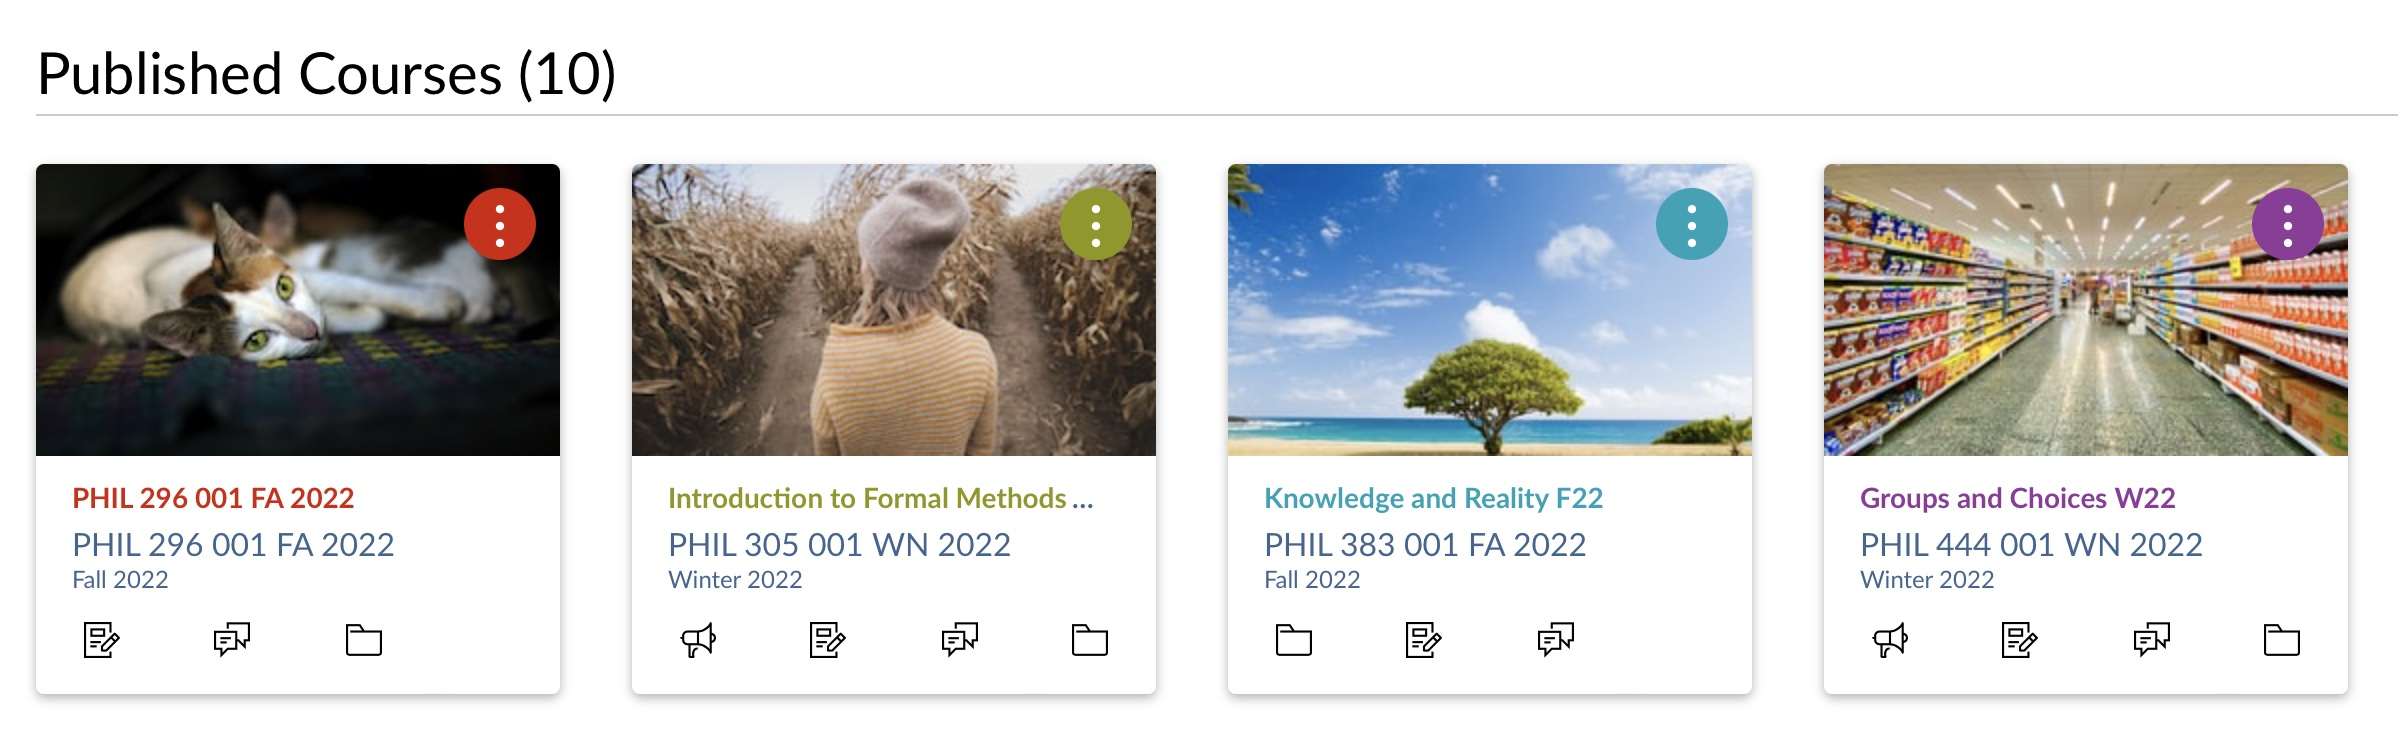
\includegraphics[width=\textwidth,height=0.6\textheight]{../images/canvas.jpeg}

}

\caption{~}

\end{figure}
\end{frame}

\begin{frame}{Syllabus}
\protect\hypertarget{syllabus}{}
\begin{figure}

{\centering 
\includegraphics[width=\textwidth,height=0.6\textheight]{../images/syllabus.jpeg}

}

\caption{~}

\end{figure}
\end{frame}

\begin{frame}{Slides}
\protect\hypertarget{slides}{}
\begin{itemize}[<+->]
\tightlist
\item
  All the slides are on Canvas.
\item
  You don't need to copy down anything that's up here.
\end{itemize}
\end{frame}

\begin{frame}{Grading}
\protect\hypertarget{grading}{}
\begin{itemize}[<+->]
\tightlist
\item
  Three essays
\item
  Three quizzes
\item
  Discussion section participation
\end{itemize}
\end{frame}

\begin{frame}{Co-authorship}
\protect\hypertarget{co-authorship}{}
\begin{itemize}[<+->]
\tightlist
\item
  Essays can be co-authored.
\item
  At most one co-author per paper.
\item
  Different co-authors for different papers.
\end{itemize}
\end{frame}

\begin{frame}{Skills}
\protect\hypertarget{skills}{}
Why are we going to read about what some 14th century dudes thought?

\begin{enumerate}[<+->]
\tightlist
\item
  Intrinsically intersting.
\item
  Cultural history.
\item
  Thinking and writing clearly about hard subjects is valuable.
\end{enumerate}
\end{frame}

\begin{frame}{An Extrinsic Payoff}
\protect\hypertarget{an-extrinsic-payoff}{}
\begin{figure}

{\centering 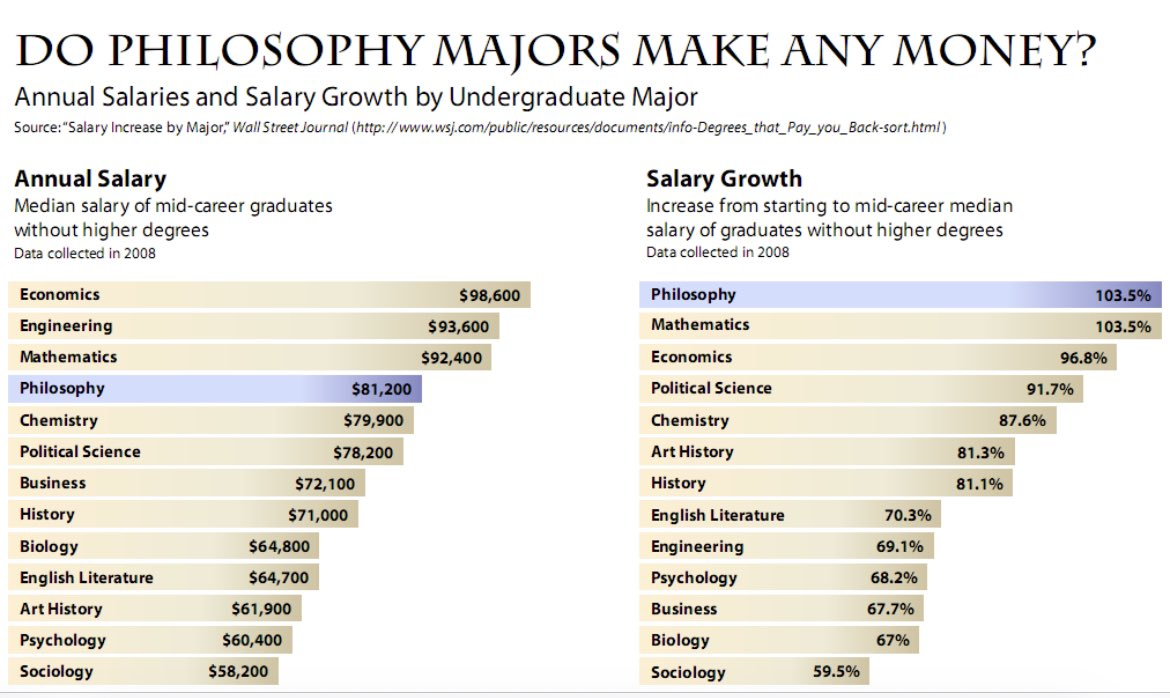
\includegraphics[width=\textwidth,height=0.7\textheight]{../images/philosophy_pay.jpeg}

}

\caption{~}

\end{figure}
\end{frame}

\begin{frame}{The Two Books We're Reading}
\protect\hypertarget{the-two-books-were-reading}{}
\begin{columns}[T]
\begin{column}{0.48\textwidth}
\begin{figure}

{\centering 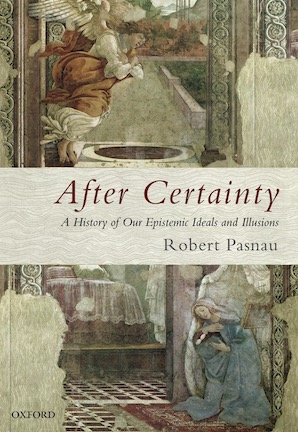
\includegraphics[width=\textwidth,height=0.6\textheight]{../images/pasnau_cover.jpeg}

}

\caption{Pasnau, After certainty}

\end{figure}
\end{column}

\begin{column}{0.48\textwidth}
\begin{figure}

{\centering 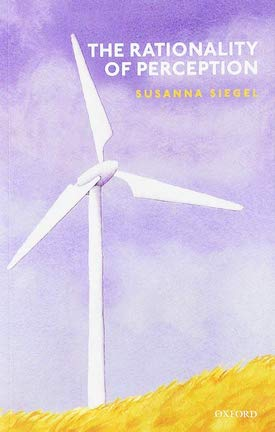
\includegraphics[width=\textwidth,height=0.6\textheight]{../images/siegel_cover.jpeg}

}

\caption{Siegel, Rationality of Perception}

\end{figure}
\end{column}
\end{columns}
\end{frame}

\hypertarget{pasnau}{%
\section{Pasnau}\label{pasnau}}

\begin{frame}{Belief}
\protect\hypertarget{belief}{}
Here are some things I believe: \pause

\begin{itemize}[<+->]
\tightlist
\item
  I have two hands.
\item
  The Battle of Gettysburg was in 1863.
\item
  Human action is causing global warming.
\end{itemize}
\end{frame}

\begin{frame}{Two Questions}
\protect\hypertarget{two-questions}{}
Two questions about each of these beliefs: \pause

\begin{enumerate}[<+->]
\tightlist
\item
  What would it take for these beliefs to be ideal, and how can we be
  more like that?
\item
  When is the belief good enough to assert/act on/hold?
\end{enumerate}
\end{frame}

\begin{frame}{Pasnau's Focus}
\protect\hypertarget{pasnaus-focus}{}
One big theme of his book:

\begin{itemize}[<+->]
\tightlist
\item
  Philosophers used to care more about the first question, but they came
  to care more about the second.
\item
  This was a mistake.
\end{itemize}
\end{frame}

\begin{frame}{The Ideal}
\protect\hypertarget{the-ideal}{}
If you like the first question, then some natural questions arise from
it.

\begin{itemize}[<+->]
\tightlist
\item
  Can we ever be epistemically ideal?
\item
  If so, in what situations can we be ideal? Is it when thinking about
  mathematics, or our own minds, or, most optimistically, the external
  world.
\end{itemize}
\end{frame}

\begin{frame}{Pasnau}
\protect\hypertarget{pasnau-1}{}
The book is primarily about two time periods:

\begin{itemize}[<+->]
\tightlist
\item
  Early 14th century; and
\item
  Late 17th century.
\end{itemize}
\end{frame}

\begin{frame}{Pasnau}
\protect\hypertarget{pasnau-2}{}
\begin{itemize}[<+->]
\tightlist
\item
  The body text, which we'll cover, is only about 1/3 of the book.
\item
  The endnotes are fascinating, and while I encourage you to read them,
  they aren't required.
\end{itemize}
\end{frame}

\begin{frame}{Pasnau}
\protect\hypertarget{pasnau-3}{}
\begin{itemize}[<+->]
\tightlist
\item
  The book is very focussed on Western Europe; mostly France and
  England.
\item
  It's a bit of a pity it didn't do more to connect the debates here to
  debates in Indian philosophy.
\end{itemize}
\end{frame}

\hypertarget{siegel}{%
\section{Siegel}\label{siegel}}

\begin{frame}{An Example}
\protect\hypertarget{an-example}{}
\begin{columns}[T]
\begin{column}{0.48\textwidth}
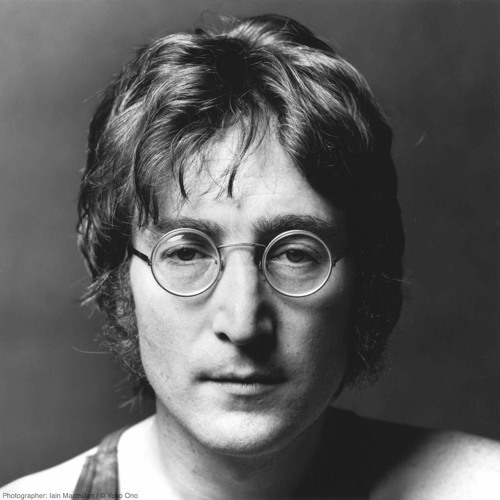
\includegraphics[width=\textwidth,height=0.7\textheight]{../images/lennon.jpeg}
\end{column}

\begin{column}{0.48\textwidth}
I'm sick and tired\\
\hspace*{0.333em}\hspace*{0.333em}of hearing things\\
From uptight, short-sighted,\\
\hspace*{0.333em}\hspace*{0.333em}narrow-minded hypocritics\\
\hspace*{0.333em}\hspace*{0.333em}\hspace*{0.333em}\hspace*{0.333em}\hspace*{0.333em}\hspace*{0.333em}\hspace*{0.333em}John
Lennon,\\
\hspace*{0.333em}\hspace*{0.333em}\hspace*{0.333em}\hspace*{0.333em}\hspace*{0.333em}\hspace*{0.333em}\hspace*{0.333em}``Gimme
Some Truth''
\end{column}
\end{columns}
\end{frame}

\begin{frame}{Two Epistemic Shortcomings}
\protect\hypertarget{two-epistemic-shortcomings}{}
\begin{enumerate}[<+->]
\item
  Short-sighted
\item
  Narrow-minded
\end{enumerate}
\end{frame}

\begin{frame}{Epistemic Vices}
\protect\hypertarget{epistemic-vices}{}
If we treat these literally,\\
\hspace*{0.333em}\hspace*{0.333em}\hspace*{0.333em}\hspace*{0.333em}narrow-mindedness
is a \textbf{vice},\\
\hspace*{0.333em}\hspace*{0.333em}\hspace*{0.333em}\hspace*{0.333em}while
short-sightedness is at worst a \textbf{misfortune}.
\end{frame}

\begin{frame}{A Simple Picture of Empirical Knowledge}
\protect\hypertarget{a-simple-picture-of-empirical-knowledge}{}
\begin{enumerate}[<+->]
\tightlist
\item
  We get inputs from reality via our perceptual system.
\item
  We use our minds to figure out more things about the world using these
  inputs.
\end{enumerate}
\end{frame}

\begin{frame}{Philosophical Differences Between Stages}
\protect\hypertarget{philosophical-differences-between-stages}{}
\begin{itemize}[<+->]
\tightlist
\item
  If dualism is true, the first is carried out by our body, the second
  by our mind.
\end{itemize}
\end{frame}

\begin{frame}{Philosophical Differences Between Stages}
\protect\hypertarget{philosophical-differences-between-stages-1}{}
\begin{itemize}[<+->]
\tightlist
\item
  Even if that's not right, philosophy has something to say about the
  second, but not really about the first.
\end{itemize}
\end{frame}

\begin{frame}{Philosophical Differences Between Stages}
\protect\hypertarget{philosophical-differences-between-stages-2}{}
\begin{itemize}[<+->]
\tightlist
\item
  Relatedly, we criticise people for doing badly at the second, but not
  the first.
\end{itemize}
\end{frame}

\begin{frame}{Some Questions}
\protect\hypertarget{some-questions}{}
\begin{enumerate}[<+->]
\tightlist
\item
  Where is the perception/inference boundary?
\item
  What are the inputs that perception provides to inference?
\item
  Does the postulation of a boundary make sense given modern biological
  theories?
\item
  Does the two-stage, dualist, picture make sense?
\end{enumerate}
\end{frame}

\begin{frame}{Two Radical Views}
\protect\hypertarget{two-radical-views}{}
\begin{itemize}[<+->]
\tightlist
\item
  Philosophical, evaluative, terms are appropriate either side of the
  boundary. We can talk about the \textbf{Rationality of Perception}.
\item
  The boundary does not in fact make sense, and should be abandoned as
  pre-scientific.
\end{itemize}
\end{frame}

\begin{frame}{Motivation for Radicalism}
\protect\hypertarget{motivation-for-radicalism}{}
Prejudiced seeing
\end{frame}

\hypertarget{four-issues-in-epistemology}{%
\section{Four Issues in
Epistemology}\label{four-issues-in-epistemology}}

\begin{frame}{Ways of Knowing}
\protect\hypertarget{ways-of-knowing}{}
\begin{itemize}[<+->]
\tightlist
\item
  How many distinct ways of knowing are there?
\item
  Is testimony one of them?
\end{itemize}
\end{frame}

\begin{frame}{Justification}
\protect\hypertarget{justification}{}
Is having a justified belief more a matter of:

\begin{itemize}[<+->]
\tightlist
\item
  Having a well-ordered mind?; or
\item
  Having a reliable connection to reality?
\end{itemize}
\end{frame}

\begin{frame}{Knowledge}
\protect\hypertarget{knowledge}{}
\begin{itemize}[<+->]
\tightlist
\item
  What is the difference betewen knowledge and lucky guesses?
\end{itemize}
\end{frame}

\begin{frame}{Scepticism}
\protect\hypertarget{scepticism}{}
\begin{itemize}[<+->]
\tightlist
\item
  Do we know anything about the external world?
\item
  If so, how and why do sceptical arguments fail?
\end{itemize}
\end{frame}

\begin{frame}{For Next Time}
\protect\hypertarget{for-next-time}{}
\begin{itemize}[<+->]
\tightlist
\item
  We will start a fair way back, with a (very quick!) survey of some
  issues that come up in Classical Indian Epistemology.
\end{itemize}
\end{frame}



\end{document}
